\clearpage
\section{\label{Run14TPC}Run14 TPC analysis}
\subsection{Datasets and Cuts}
In this Run14 $D^0$ TPC analysis, we ran 667 million events ($\sim$62\% of total). Cuts are listed in the following.
\begin{itemize}
\item \textbf{Library}: P16id.

\item \textbf{Trigger IDs}:  450050, 450060, 450005, 450015, 450025.

\item \textbf{Centrality}: 0-80\%.

\item \textbf{Vertex selections}
\begin{itemize}
\item $|v_z^{TPC}| < 6$ cm
\item $|v_z^{TPC} - v_z^{VPD}| < 3$ cm
\end{itemize}

\item \textbf{Track selections}
\begin{itemize}
\item $p_T > 0.2$ GeV/c
\item $|\eta| < 1$
\item $\mathrm{global ~ DCA} < 1$ cm
\item $20 \leq \mathrm{nHitsFit} < 50$
\item $\mathrm{nHitsFit}/\mathrm{nHitsMax} > 0.52$
\item $\mathrm{nHitsdEdx} > 15$
\end{itemize}

\item \textbf{PID}
\begin{itemize}
\item TPC PID (dE/dx): $|n\sigma_K| < 2$ and $|n\sigma_\pi| < 2$
\item TOF PID (1/$\beta$): define $n\sigma_X^{TOF} = ( \frac{1}{\beta} - \sqrt{m_X^2/p^2 + 1} )/\sigma + c$, here $\sigma = 0.013$, $c = 0$,  $m_X$ is particle ($K$, $\pi$, etc.) mass. For pions, we apply $-2.0 < n\sigma_\pi^{TOF} < f_\pi^{\mathrm{max}}(p)$, here
\begin{equation}
f_\pi^{\mathrm{max}}(p) = \left\{
\begin{aligned}
&5.43 - 2.14x, ~ p < 1.6  \\
&2, ~ p \geq 1.6
\end{aligned}
\right.
\label{eq:Run14nsigTofPi}
\end{equation}
For kaons, we apply $f_K^{\mathrm{min}}(p) < n\sigma_K^{TOF} < f_K^{\mathrm{max}}(p)$, here
\begin{equation}
f_K^{\mathrm{min}}(p) = \left\{
\begin{aligned}
&-7.54 + 5.83p - 1.31p^2, ~ p < 1.37  \\
&-2, ~ p \geq 1.37
\end{aligned}
\right.
\label{eq:Run14nsigTofK1}
\end{equation}

\begin{equation}
f_K^{\mathrm{max}}(p) = \left\{
\begin{aligned}
&8.69 - 6.02p + 1.32p^2, ~ p < 1.9  \\
&2, ~ p \geq 1.9
\end{aligned}
\right.
\label{eq:Run14nsigTofK1}
\end{equation}

There are two PID cases:
\begin{itemize}
\item hybrid PID: Apply TOF PID while TOF is available (TOFMatchFlag $>$ 0 \&\& $\beta > 0$ \&\& $|\mathrm{ylocal}| < 1.8$) , otherwise use TPC PID only.
\item clean PID: It's the same as hybrid PID, except that TOF must be used at $p < 1.6$ GeV/c (TOFMatchFlag $>$ 0 \&\& $\beta > 0$ \&\& $|\mathrm{ylocal}| < 1.8$). 
\end{itemize}
\end{itemize}

\item \textbf{$D^0$ rapidity}: $|y| < 1$.
\end{itemize}

\subsection{$D^0$ recronstruction}
We reconstruct $D^0$ through the channel $D^0 \rightarrow K^-\pi^+$(B.R. = 0.0388). Background is reconstructed with mix-event method. 9 centrality bins (0-80\%), 4 primary vertex $v_z$ bins ($v_z \in [-6,6]$ cm) and 12 event plane bins ($\Psi_2 \in [0,\pi]$) are used to classify mixed events with some degree of similarity. Mix-event unlike-sign background is scaled to same-event like-sign background at the mass region of $1.69 < \mathrm{mass}_{K\pi} < 2.04$ GeV/$c^2$. Then same event unlike-sign (signal + background) subtracted by scaled mix-event unlike-sign background are fitted with a gaussian function (signal) plus a second order polynomial function (residual background). The fit range is 1.69-2.04 GeV/$c^2$.

Fig.~\ref{fig:Run14TpcClean0_80} shows $D^0$ signal at 6 $p_T$ bins (0-0.7, 0.7-1.1, 1.1-1.6, 1.6-2.2, 2.2-3.0, 3.0-5.0) in 0-80\% with clean PID.
\begin{figure}
    \centering
    \subfigure{\includegraphics[width=0.32\textwidth]{{figure/Run14TPC/ptDivision1/cleanPID/cent0_80_pt_0.0_0.7}.eps}}
    \subfigure{\includegraphics[width=0.32\textwidth]{{figure/Run14TPC/ptDivision1/cleanPID/cent0_80_pt_0.7_1.1}.eps}}
    \subfigure{\includegraphics[width=0.32\textwidth]{{figure/Run14TPC/ptDivision1/cleanPID/cent0_80_pt_1.1_1.6}.eps}} \\
    \subfigure{\includegraphics[width=0.32\textwidth]{{figure/Run14TPC/ptDivision1/cleanPID/cent0_80_pt_1.6_2.2}.eps}} 
    \subfigure{\includegraphics[width=0.32\textwidth]{{figure/Run14TPC/ptDivision1/cleanPID/cent0_80_pt_2.2_3.0}.eps}}
    \subfigure{\includegraphics[width=0.32\textwidth]{{figure/Run14TPC/ptDivision1/cleanPID/cent0_80_pt_3.0_5.0}.eps}}
    \caption{$D^0$ signal at 6 $p_T$ bins (0-0.7, 0.7-1.1, 1.1-1.6, 1.6-2.2, 2.2-3.0, 3.0-5.0) in 0-80\% with clean PID.}
   \label{fig:Run14TpcClean0_80}
\end{figure}

Fig.~\ref{fig:Run14TpcHybrid0_80} shows $D^0$ signal at 6 $p_T$ bins (0-0.7, 0.7-1.1, 1.1-1.6, 1.6-2.2, 2.2-3.0, 3.0-5.0) in 0-80\% with hybrid PID.
\begin{figure}
    \centering
    \subfigure{\includegraphics[width=0.32\textwidth]{{figure/Run14TPC/ptDivision1/hybridPID/cent0_80_pt_0.0_0.7}.eps}}
    \subfigure{\includegraphics[width=0.32\textwidth]{{figure/Run14TPC/ptDivision1/hybridPID/cent0_80_pt_0.7_1.1}.eps}}
    \subfigure{\includegraphics[width=0.32\textwidth]{{figure/Run14TPC/ptDivision1/hybridPID/cent0_80_pt_1.1_1.6}.eps}} \\
    \subfigure{\includegraphics[width=0.32\textwidth]{{figure/Run14TPC/ptDivision1/hybridPID/cent0_80_pt_1.6_2.2}.eps}} 
    \subfigure{\includegraphics[width=0.32\textwidth]{{figure/Run14TPC/ptDivision1/hybridPID/cent0_80_pt_2.2_3.0}.eps}}
    \subfigure{\includegraphics[width=0.32\textwidth]{{figure/Run14TPC/ptDivision1/hybridPID/cent0_80_pt_3.0_5.0}.eps}}
    \caption{$D^0$ signal at 6 $p_T$ bins (0-0.7, 0.7-1.1, 1.1-1.6, 1.6-2.2, 2.2-3.0, 3.0-5.0) in 0-80\% with hybrid PID.}
   \label{fig:Run14TpcHybrid0_80}
\end{figure}

Fig.~\ref{fig:Run14TpcClean} shows $D^0$ signal at 2 $p_T$ bins (0-2, 2-4) and 4 centralilties (0-80\%, 0-10\%, 10-40\%, 40-80\%) with clean PID.
\begin{figure}
    \centering
    \subfigure{\includegraphics[width=0.32\textwidth]{{figure/Run14TPC/cleanPID/cent0_80_pt_0.0_2.0}.eps}}
    \subfigure{\includegraphics[width=0.32\textwidth]{{figure/Run14TPC/cleanPID/cent0_80_pt_2.0_4.0}.eps}}
    \subfigure{\includegraphics[width=0.32\textwidth]{{figure/Run14TPC/cleanPID/cent0_10_pt_0.0_2.0}.eps}}  \\
    \subfigure{\includegraphics[width=0.32\textwidth]{{figure/Run14TPC/cleanPID/cent0_10_pt_2.0_4.0}.eps}} 
    \subfigure{\includegraphics[width=0.32\textwidth]{{figure/Run14TPC/cleanPID/cent10_40_pt_0.0_2.0}.eps}}
    \subfigure{\includegraphics[width=0.32\textwidth]{{figure/Run14TPC/cleanPID/cent10_40_pt_2.0_4.0}.eps}} \\
    \subfigure{\includegraphics[width=0.32\textwidth]{{figure/Run14TPC/cleanPID/cent40_80_pt_0.0_2.0}.eps}}
    \subfigure{\includegraphics[width=0.32\textwidth]{{figure/Run14TPC/cleanPID/cent40_80_pt_2.0_4.0}.eps}}
    \caption{$D^0$ signal at 2 $p_T$ bins (0-2, 2-4) and 4 centralilties (0-80\%, 0-10\%, 10-40\%, 40-80\%) with clean PID.}
   \label{fig:Run14TpcClean}
\end{figure}

Fig.~\ref{fig:Run14TpcHybrid} shows $D^0$ signal at 2 $p_T$ bins (0-2, 2-4) and 4 centralilties (0-80\%, 0-10\%, 10-40\%, 40-80\%) with hybrid PID.
\begin{figure}
    \centering
    \subfigure{\includegraphics[width=0.32\textwidth]{{figure/Run14TPC/hybridPID/cent0_80_pt_0.0_2.0}.eps}}
    \subfigure{\includegraphics[width=0.32\textwidth]{{figure/Run14TPC/hybridPID/cent0_80_pt_2.0_4.0}.eps}}
    \subfigure{\includegraphics[width=0.32\textwidth]{{figure/Run14TPC/hybridPID/cent0_10_pt_0.0_2.0}.eps}}  \\
    \subfigure{\includegraphics[width=0.32\textwidth]{{figure/Run14TPC/hybridPID/cent0_10_pt_2.0_4.0}.eps}} 
    \subfigure{\includegraphics[width=0.32\textwidth]{{figure/Run14TPC/hybridPID/cent10_40_pt_0.0_2.0}.eps}}
    \subfigure{\includegraphics[width=0.32\textwidth]{{figure/Run14TPC/hybridPID/cent10_40_pt_2.0_4.0}.eps}} \\
    \subfigure{\includegraphics[width=0.32\textwidth]{{figure/Run14TPC/hybridPID/cent40_80_pt_0.0_2.0}.eps}}
    \subfigure{\includegraphics[width=0.32\textwidth]{{figure/Run14TPC/hybridPID/cent40_80_pt_2.0_4.0}.eps}}
    \caption{$D^0$ signal at 2 $p_T$ bins (0-2, 2-4) and 4 centralilties (0-80\%, 0-10\%, 10-40\%, 40-80\%) with hybrid PID.}
   \label{fig:Run14TpcHybrid}
\end{figure}

\subsection{Efficiency and acceptance correction}
The efficiency and acceptance correction includes the following:
\begin{itemize}
\item Acceptance, including $p_T$ and $\eta$ cut efficiency.
\item TPC tracking efficiency, including the basic track quality cut efficiency (nHitsFit, ndEdxHits, nHitsRatio, gDca).
\item TOF matching efficiency.
\item PID efficiency, including TOF PID and TPC PID efficiency.
\end{itemize}

TPC tracking efficiency is obtained from $K/\pi$ embedding, showed in Fig.~\ref{fig:Run14TpcTrack}.
\begin{figure}
    \centering
    \subfigure{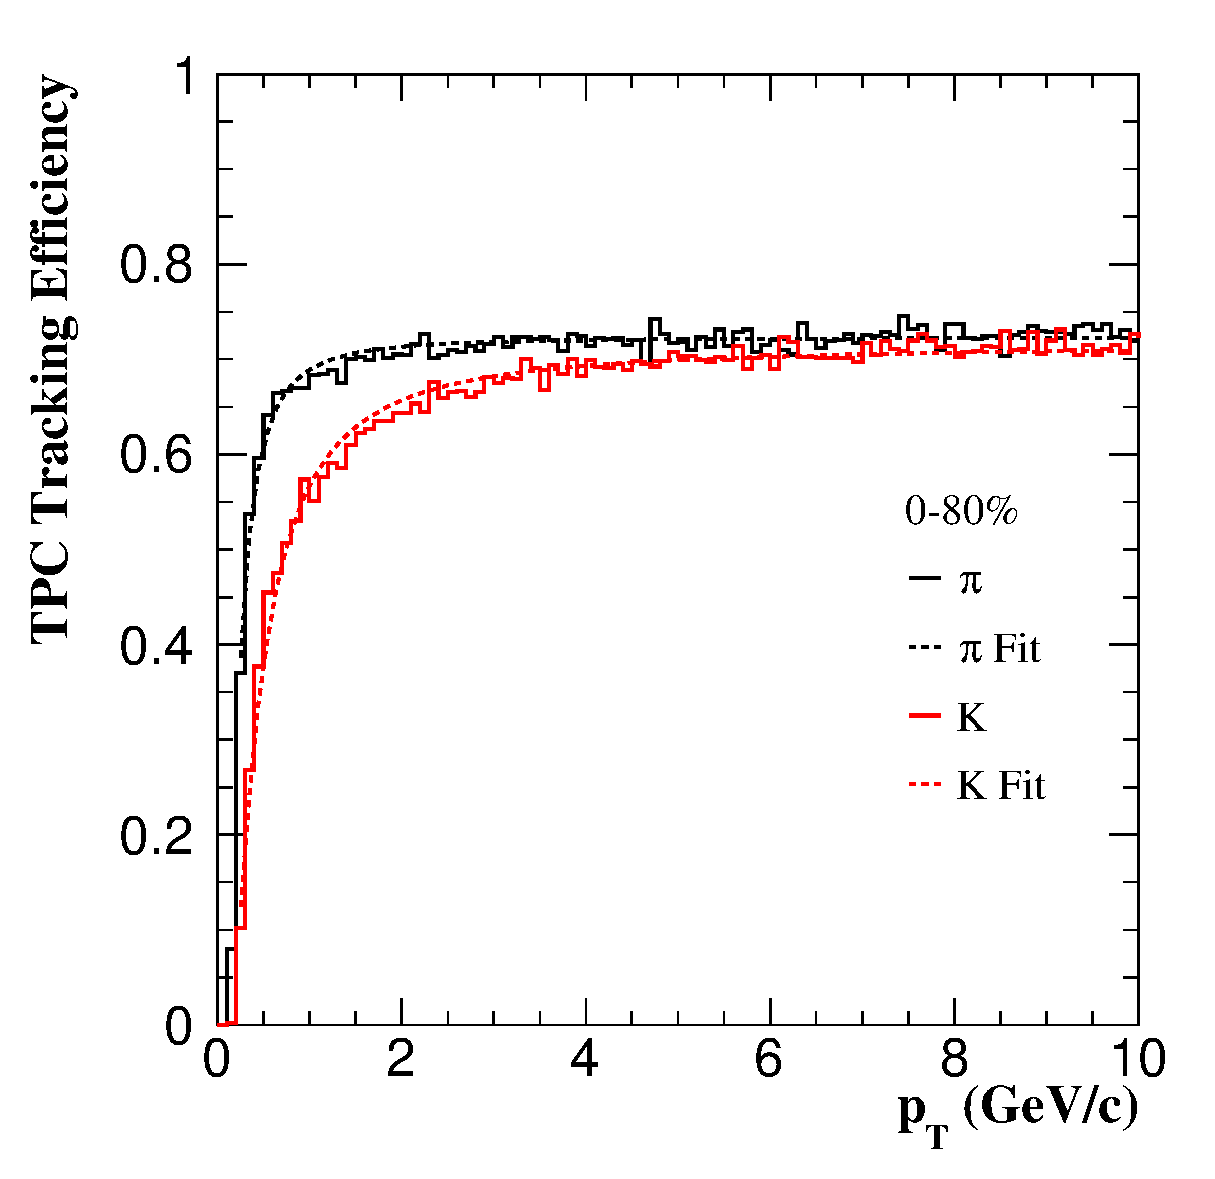
\includegraphics[width=0.47\textwidth]{{figure/Run14TPC/efficiency/tpcTrackEff_0_80}.eps}}
    \subfigure{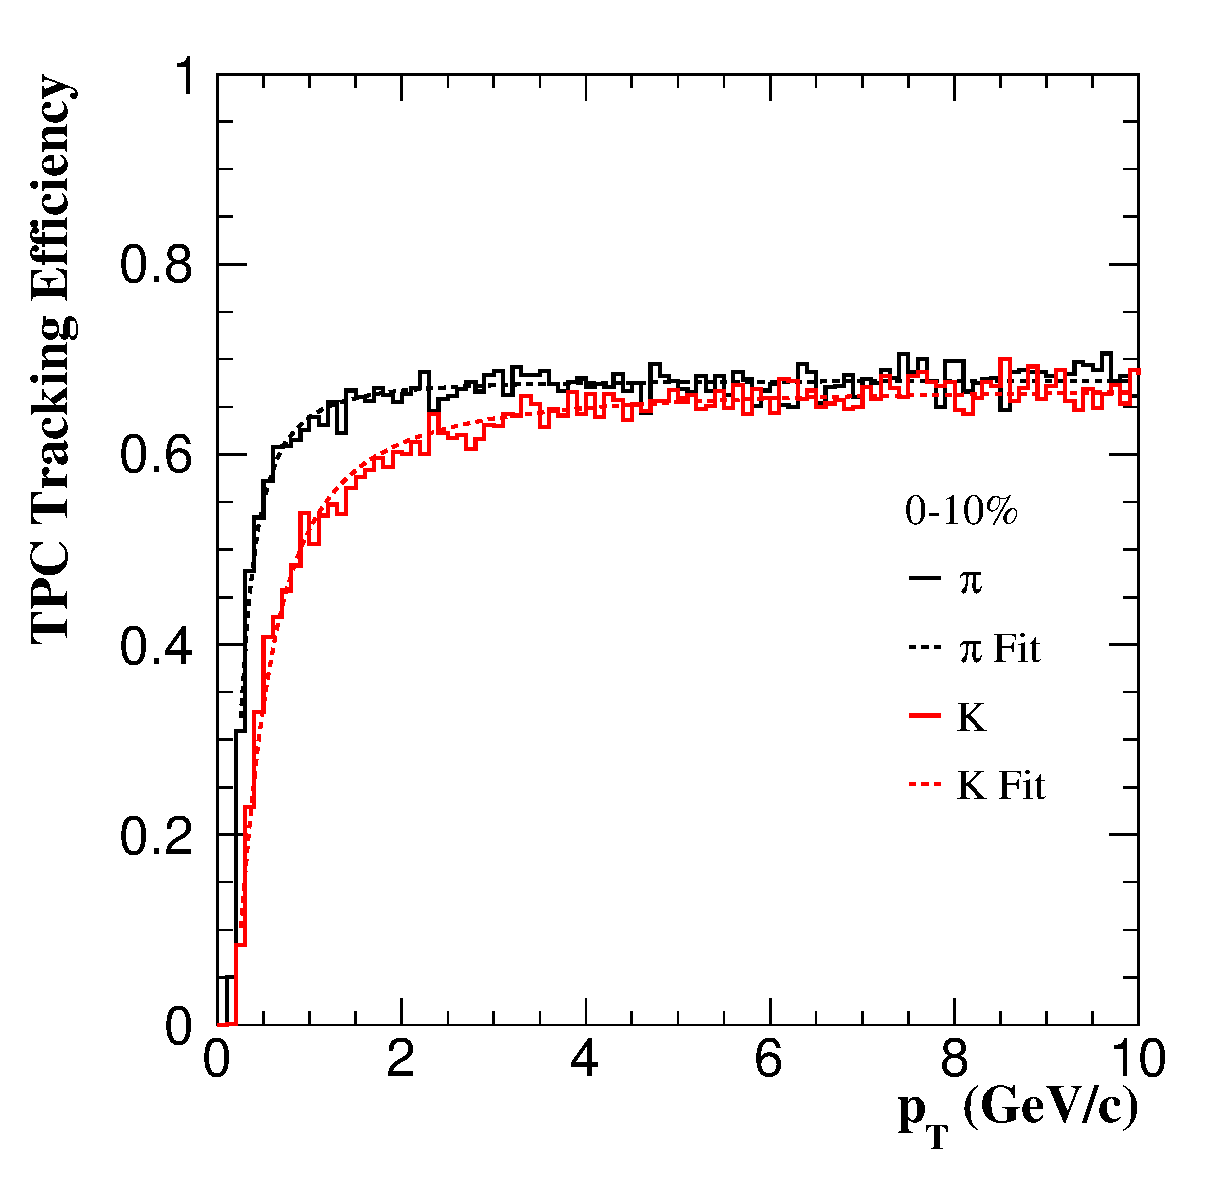
\includegraphics[width=0.47\textwidth]{{figure/Run14TPC/efficiency/tpcTrackEff_0_10}.eps}}
    \subfigure{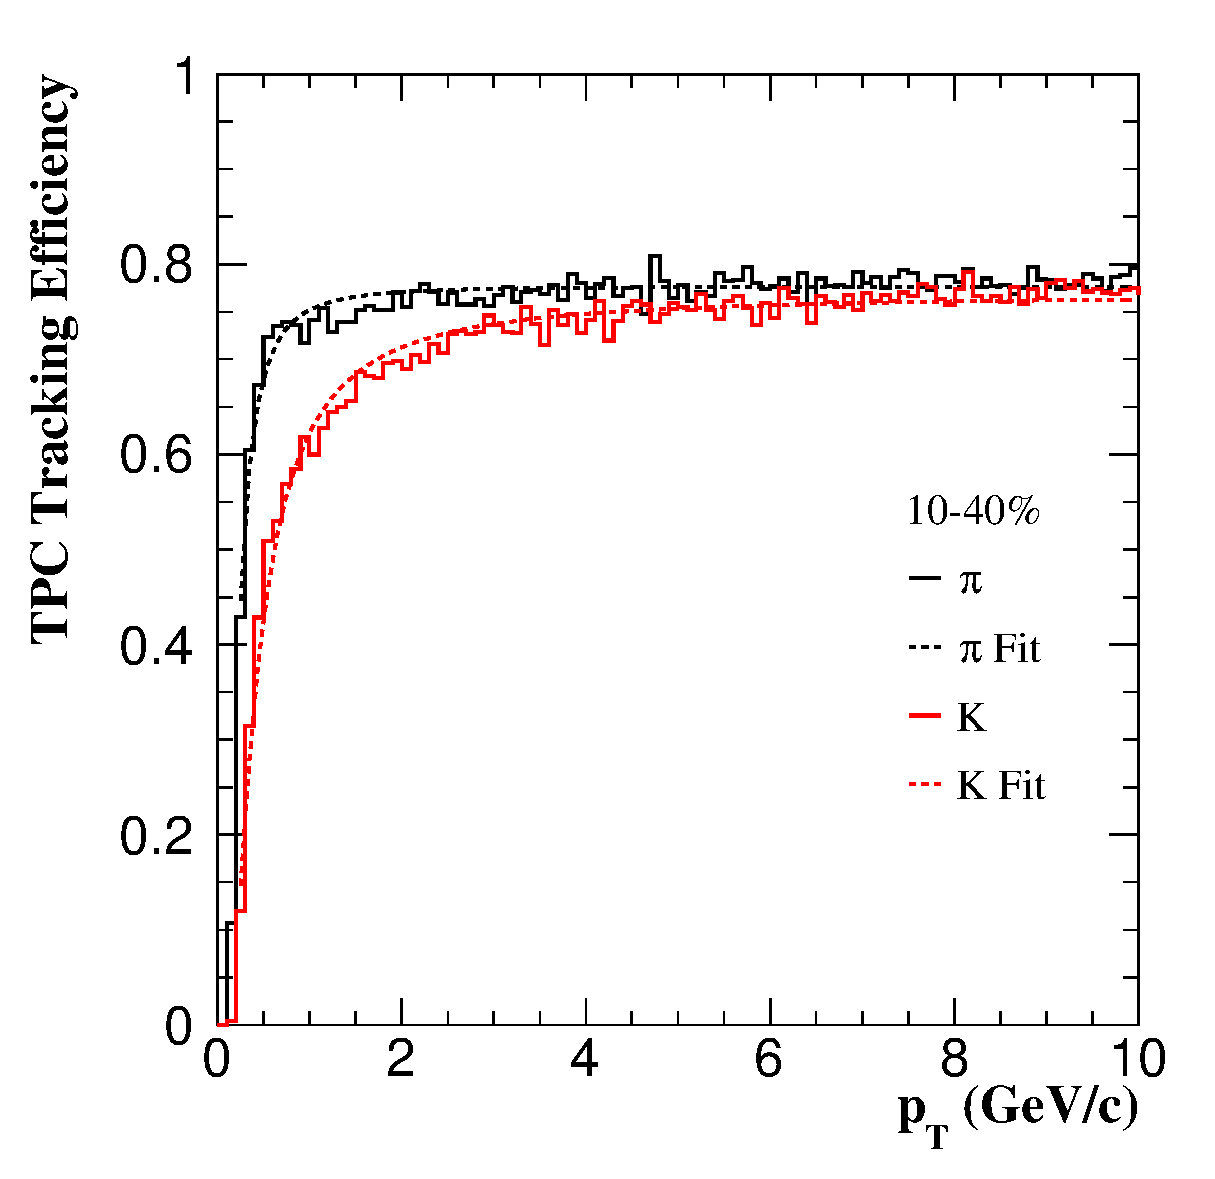
\includegraphics[width=0.47\textwidth]{{figure/Run14TPC/efficiency/tpcTrackEff_10_40}.eps}}
    \subfigure{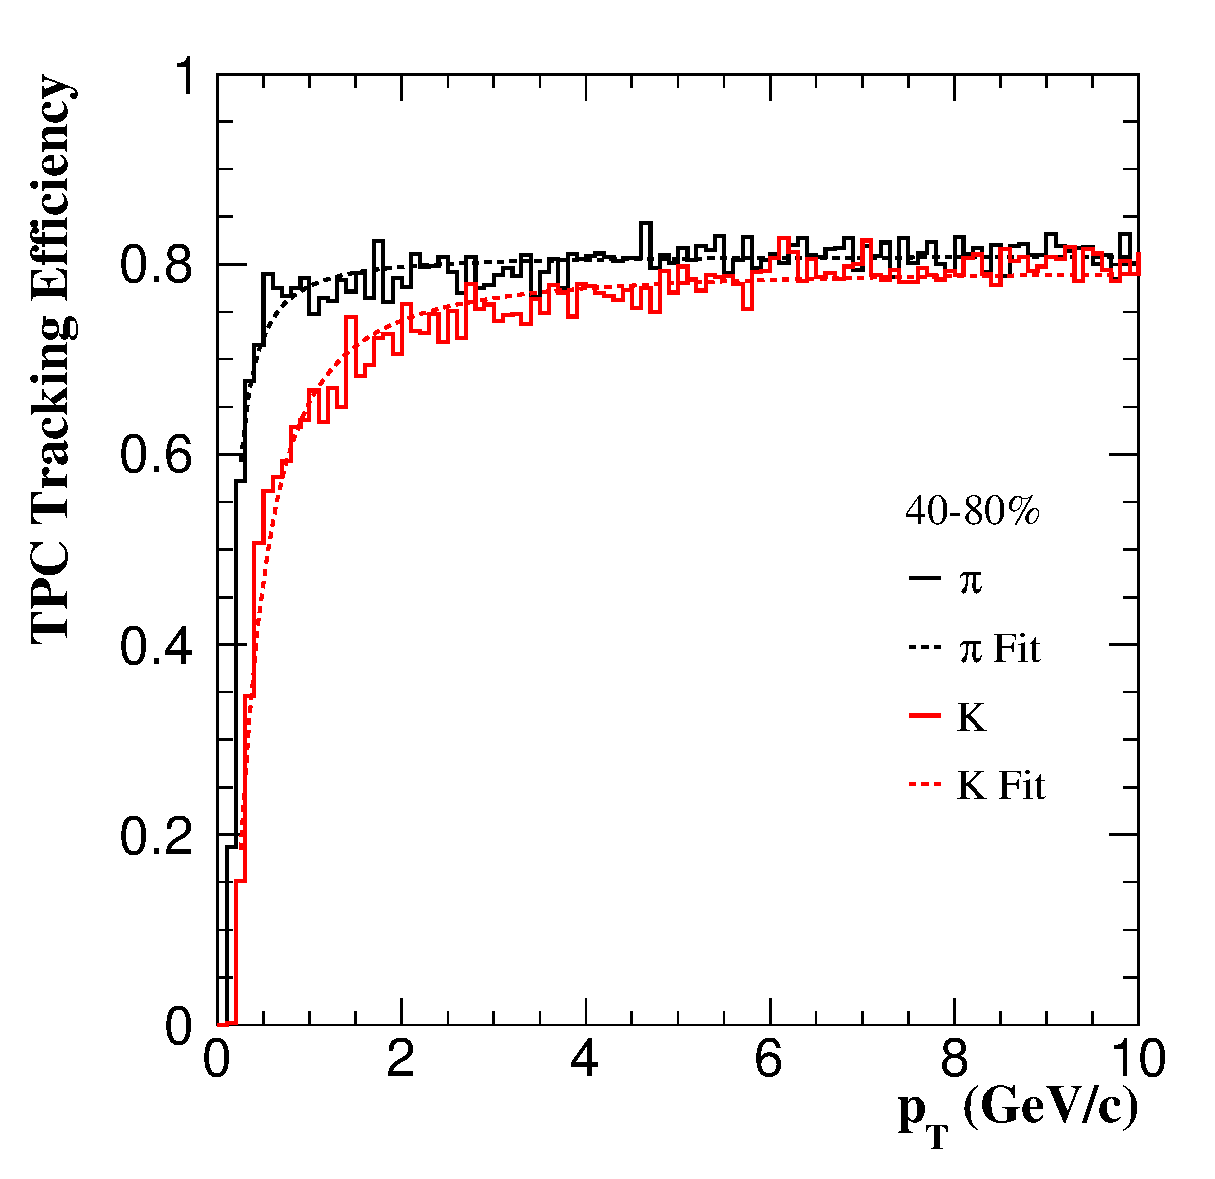
\includegraphics[width=0.47\textwidth]{{figure/Run14TPC/efficiency/tpcTrackEff_40_80}.eps}}
    \caption{Run14 TPC tracking efficiency.}
   \label{fig:Run14TpcTrack}
\end{figure}

Fig.~\ref{fig:Run14TofMatch} shows $K/\pi$ TOF matching efficiency at 0-80\%, 0-10\%, 10-40\%, 40-80\%. The dip at the $p_{T}$ region of 0.5-0.9 GeV/c for kaons is due that we use $n\sigma_{K/\pi}$ to identify $K/\pi$ and $n\sigma_K$ resolution get better at low $p_T$ when TOF match is required. Detailed validation can be found at Section~\ref{sec:TOFmatch}.
\begin{figure}
    \centering
    \subfigure{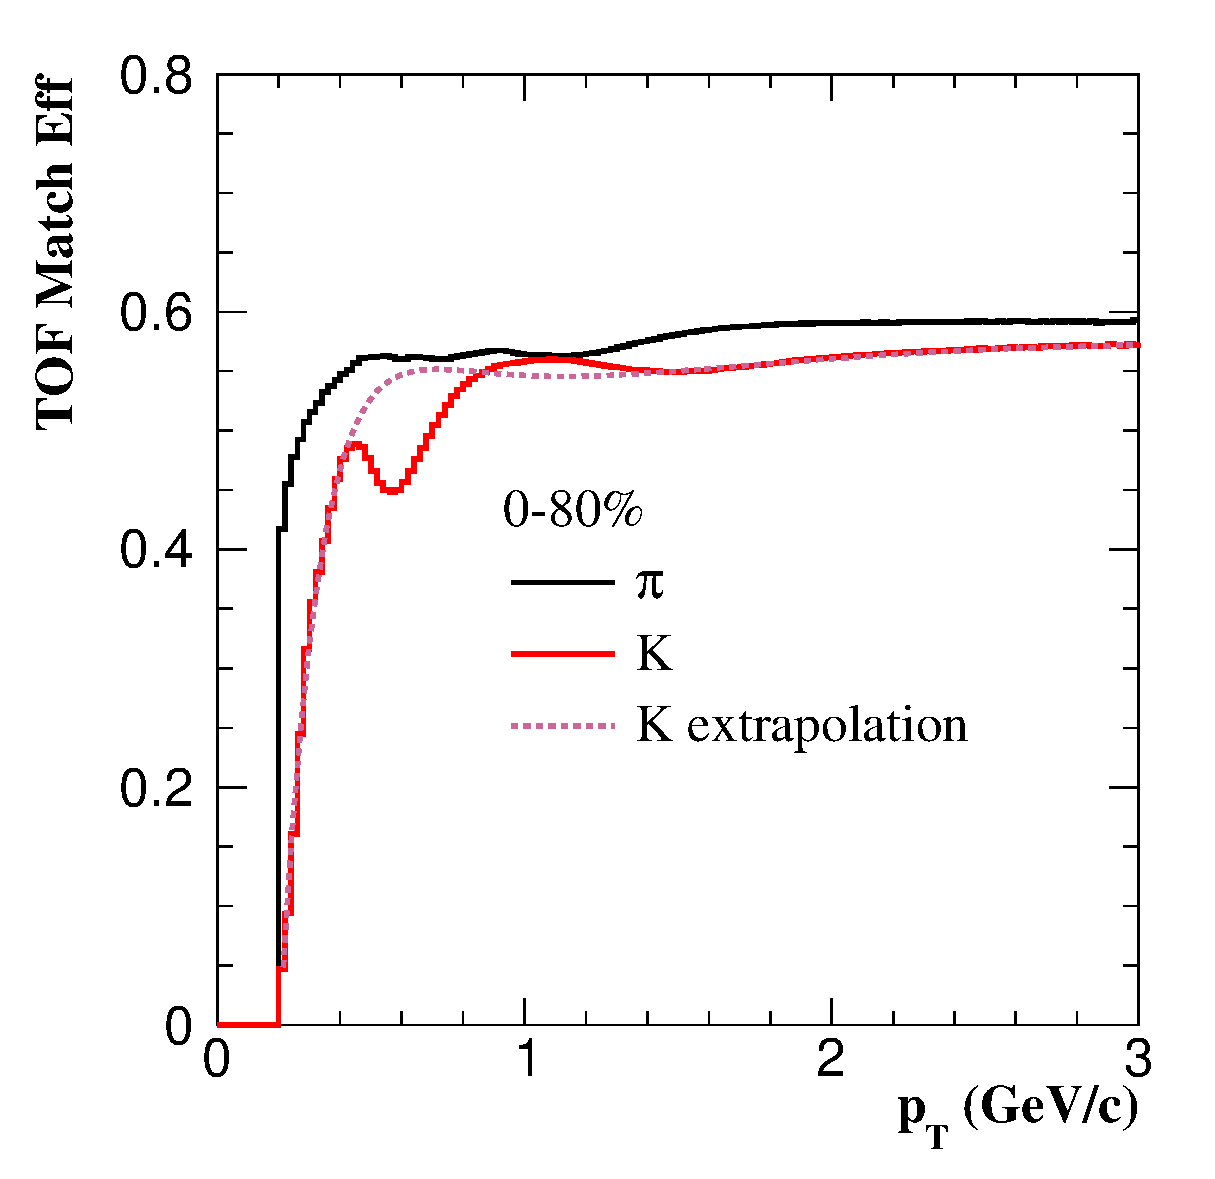
\includegraphics[width=0.47\textwidth]{{figure/Run14TPC/efficiency/tofMatchRun14_0_80}.eps}}
    \subfigure{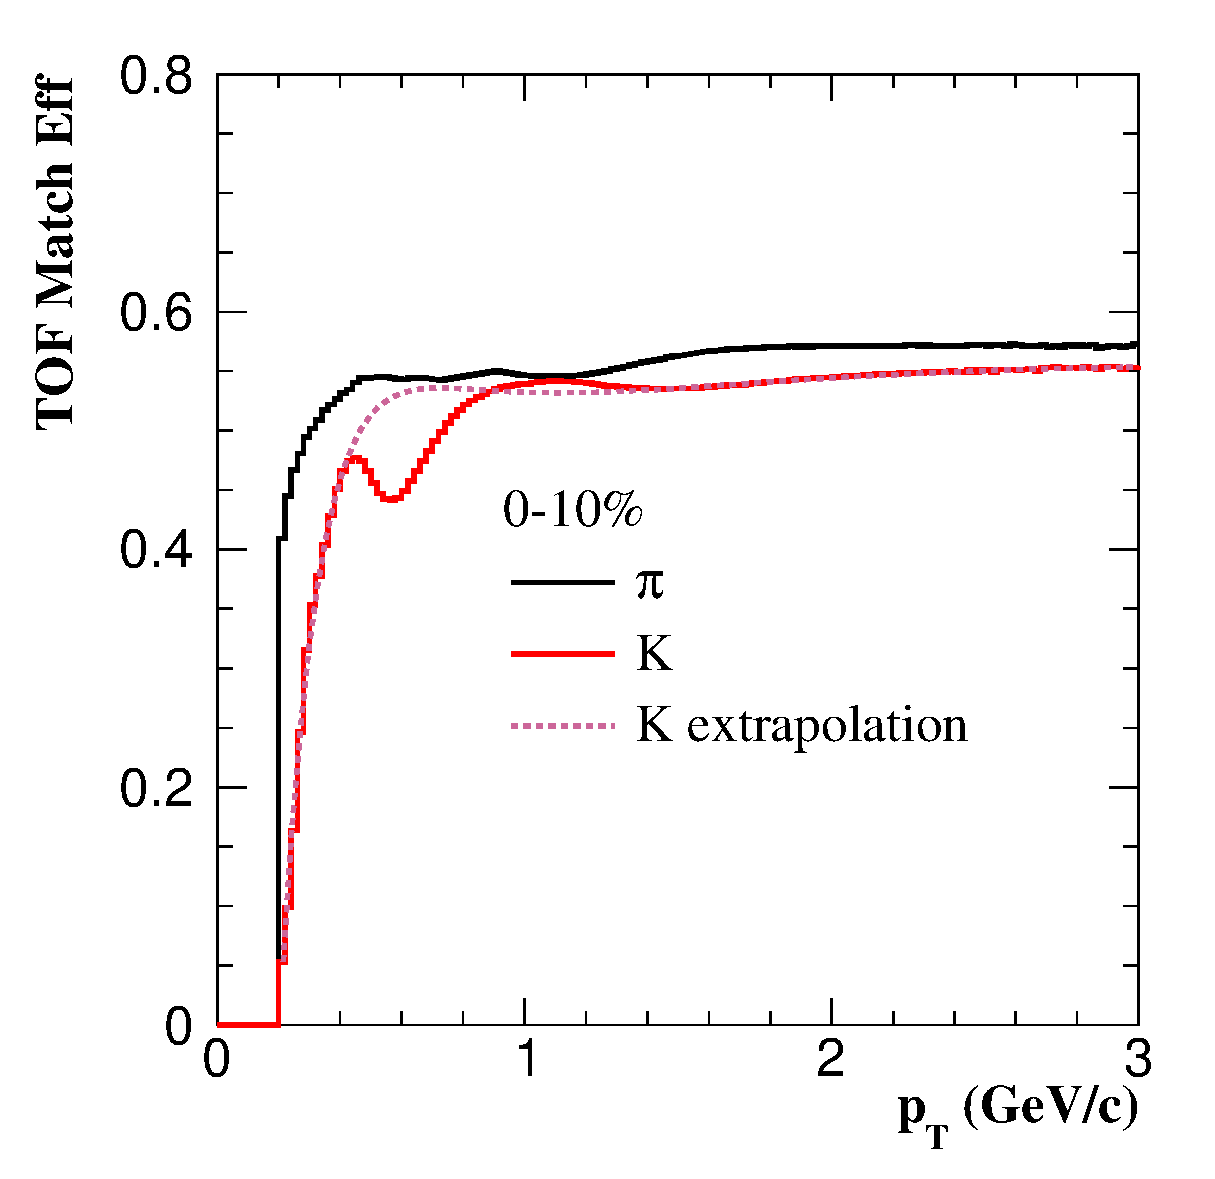
\includegraphics[width=0.47\textwidth]{{figure/Run14TPC/efficiency/tofMatchRun14_0_10}.eps}} \\
    \subfigure{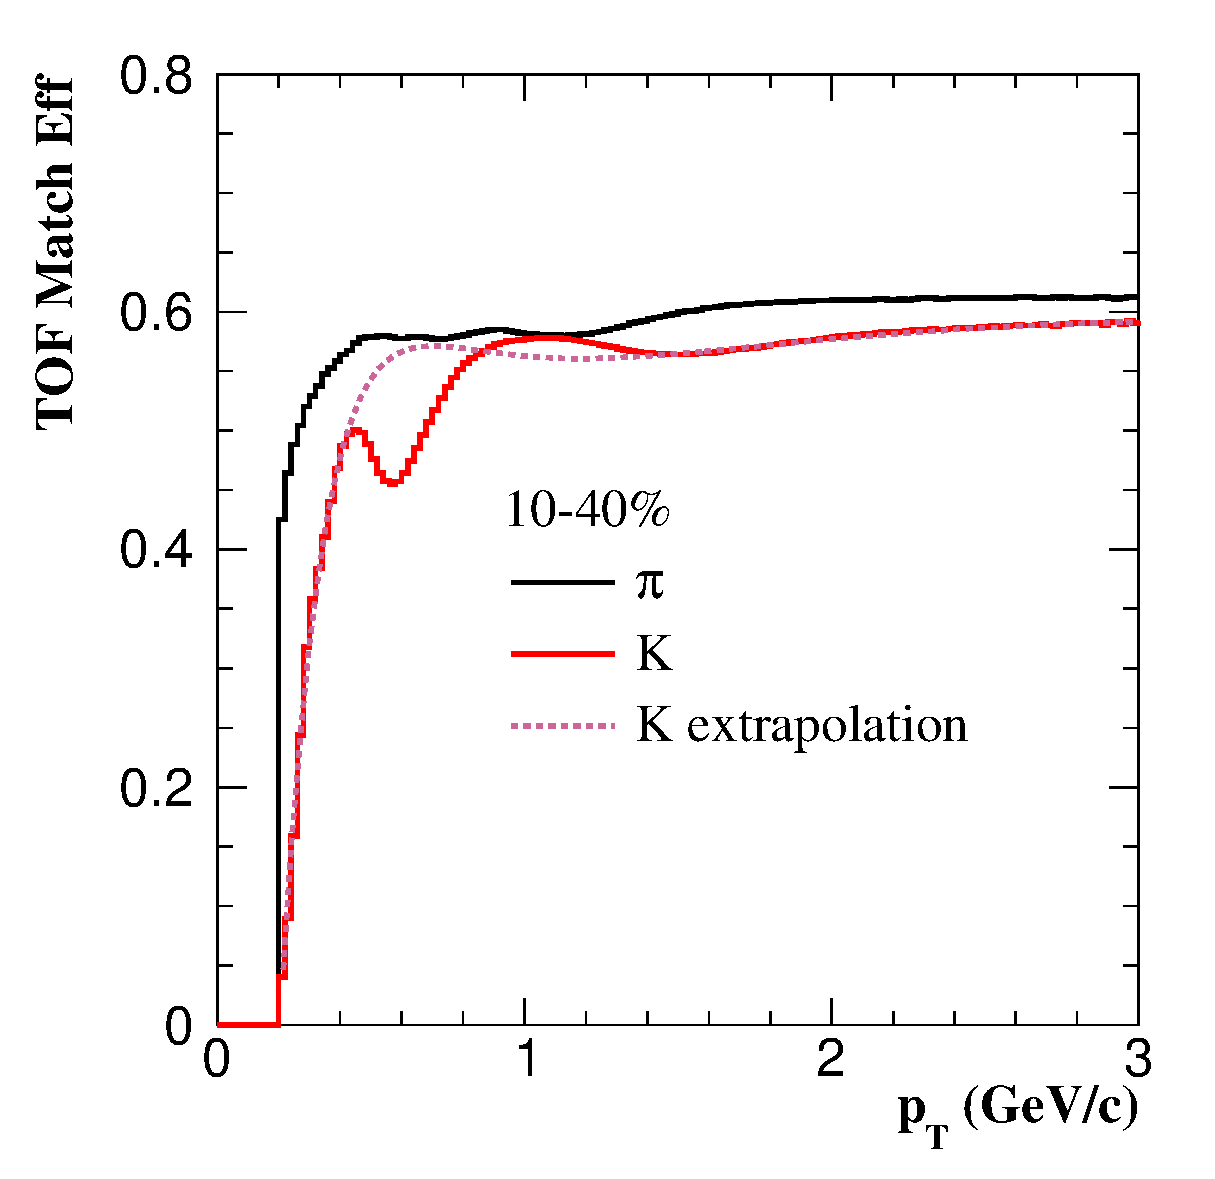
\includegraphics[width=0.47\textwidth]{{figure/Run14TPC/efficiency/tofMatchRun14_10_40}.eps}}
    \subfigure{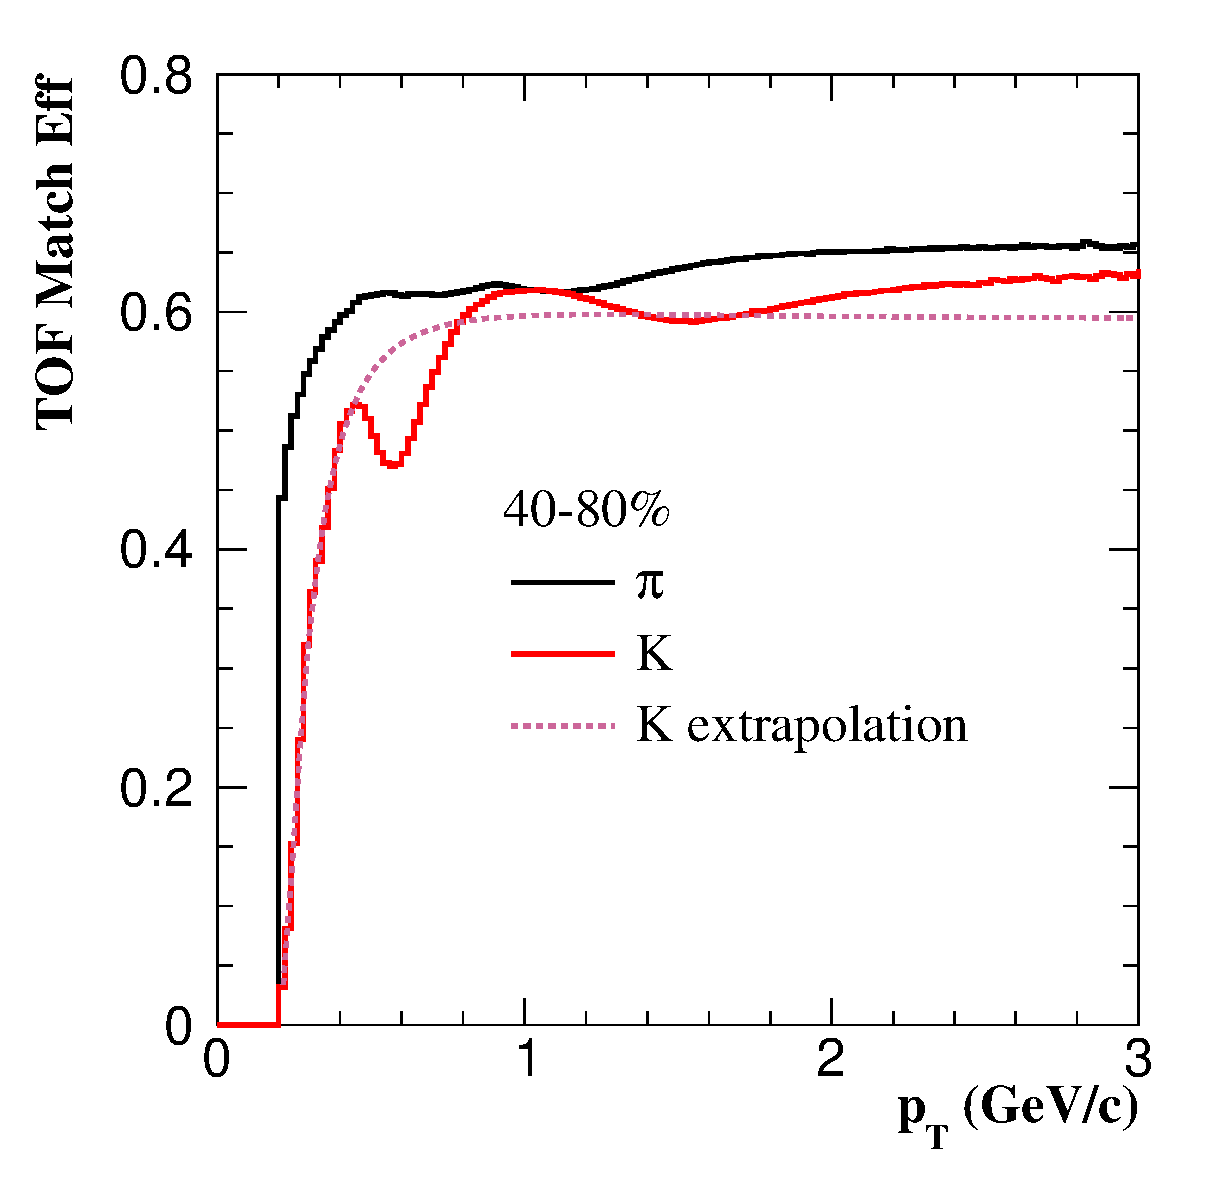
\includegraphics[width=0.47\textwidth]{{figure/Run14TPC/efficiency/tofMatchRun14_40_80}.eps}}
    \caption{Run14 $K/\pi$ TOF matching efficiency at 0-80\%, 0-10\%, 10-40\%, 40-80\%.}
   \label{fig:Run14TofMatch}
\end{figure}

Fig.~\ref{fig:Run14PidEff} shows $K/\pi$ PID efficiency. Top panels are $K/\pi$ TPC PID efficiency and bottom panels are $K/\pi$ TOF PID efficiency. Pure pions are obtained by reconstructing $K_S^0$ ($K_S^0 \rightarrow \pi^+\pi^-$) and pure kaons are obtained by reconstructing $\phi$ ($\phi \rightarrow K^+K^-$). Detailed information can be found at \url{https://drupal.star.bnl.gov/STAR/system/files/Pid_eff_new.pdf}.
\begin{figure}
    \centering
    \subfigure{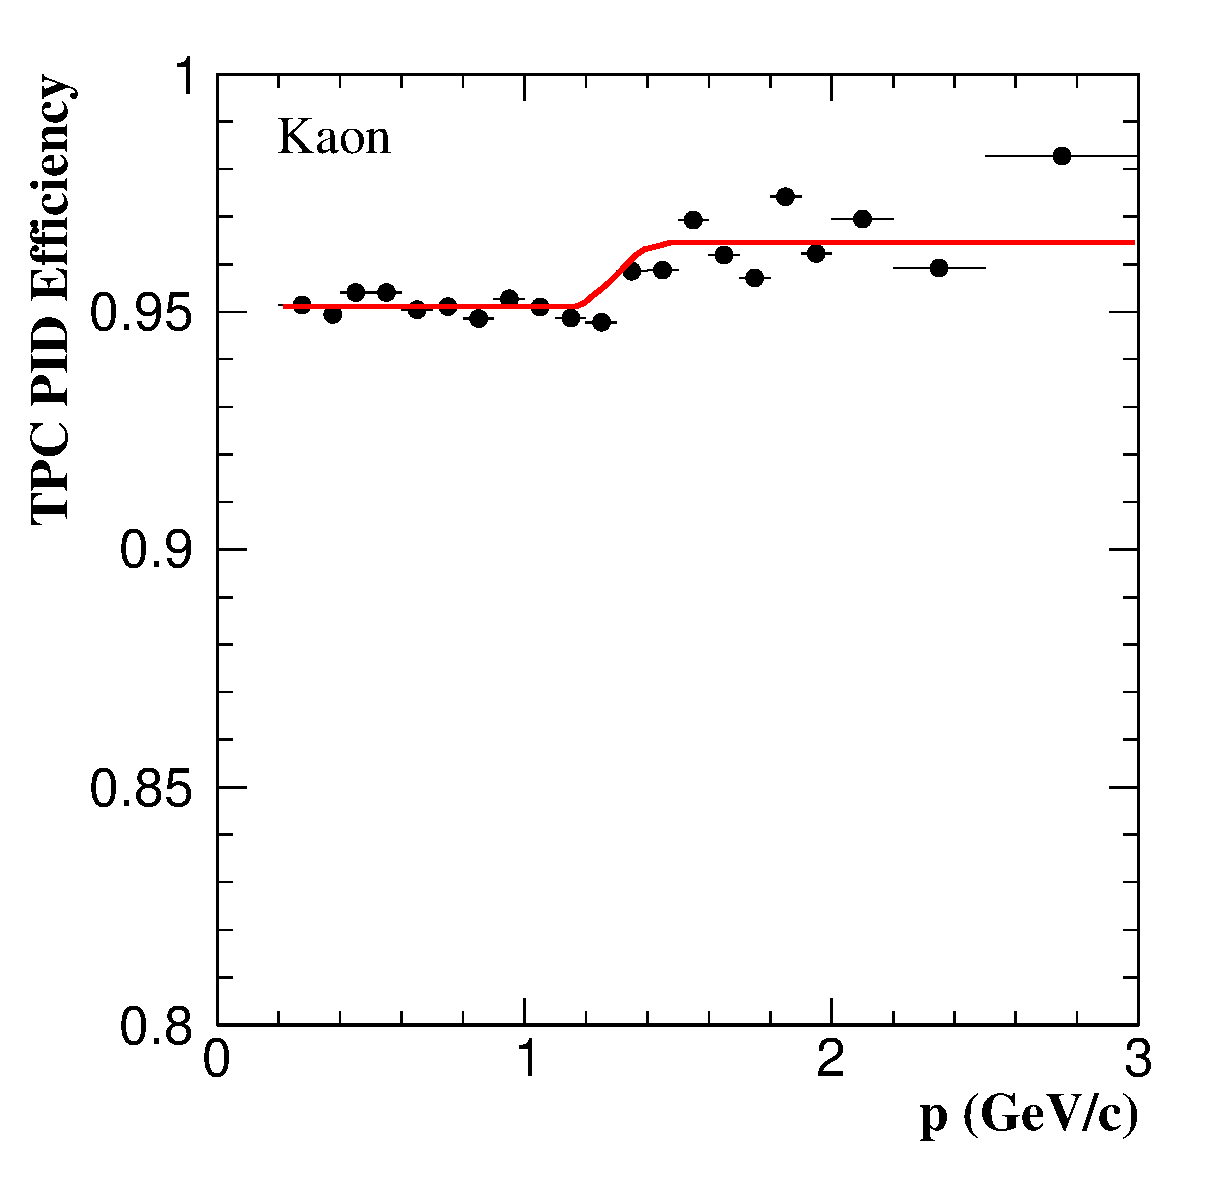
\includegraphics[width=0.47\textwidth]{{figure/Run14TPC/efficiency/kTpcPid}.eps}}
    \subfigure{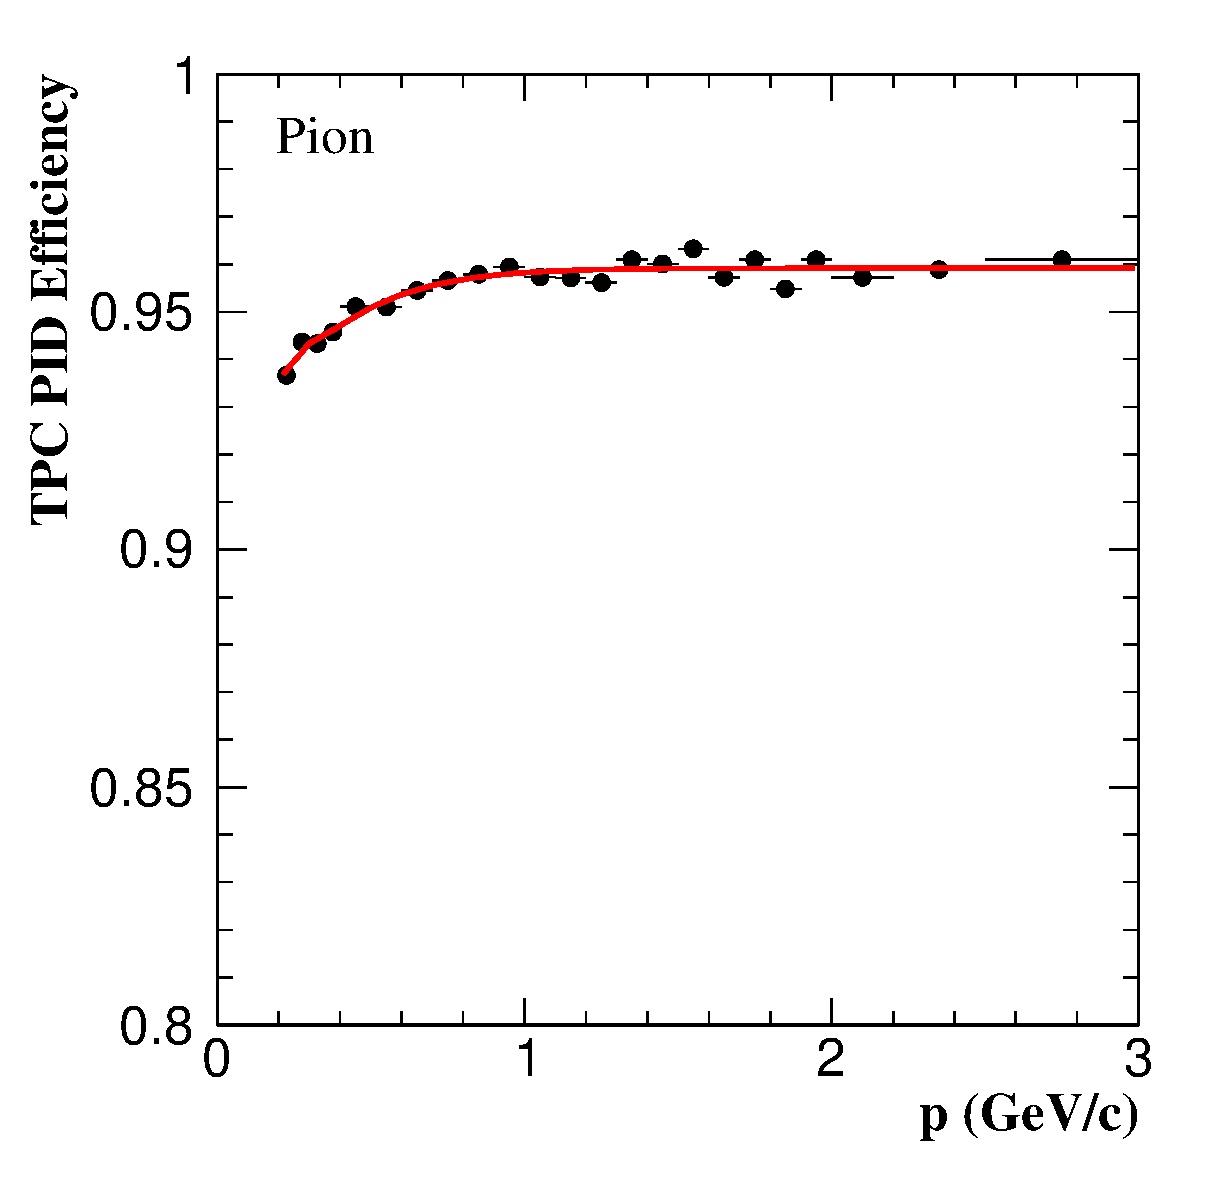
\includegraphics[width=0.47\textwidth]{{figure/Run14TPC/efficiency/piTpcPid}.eps}} \\
    \subfigure{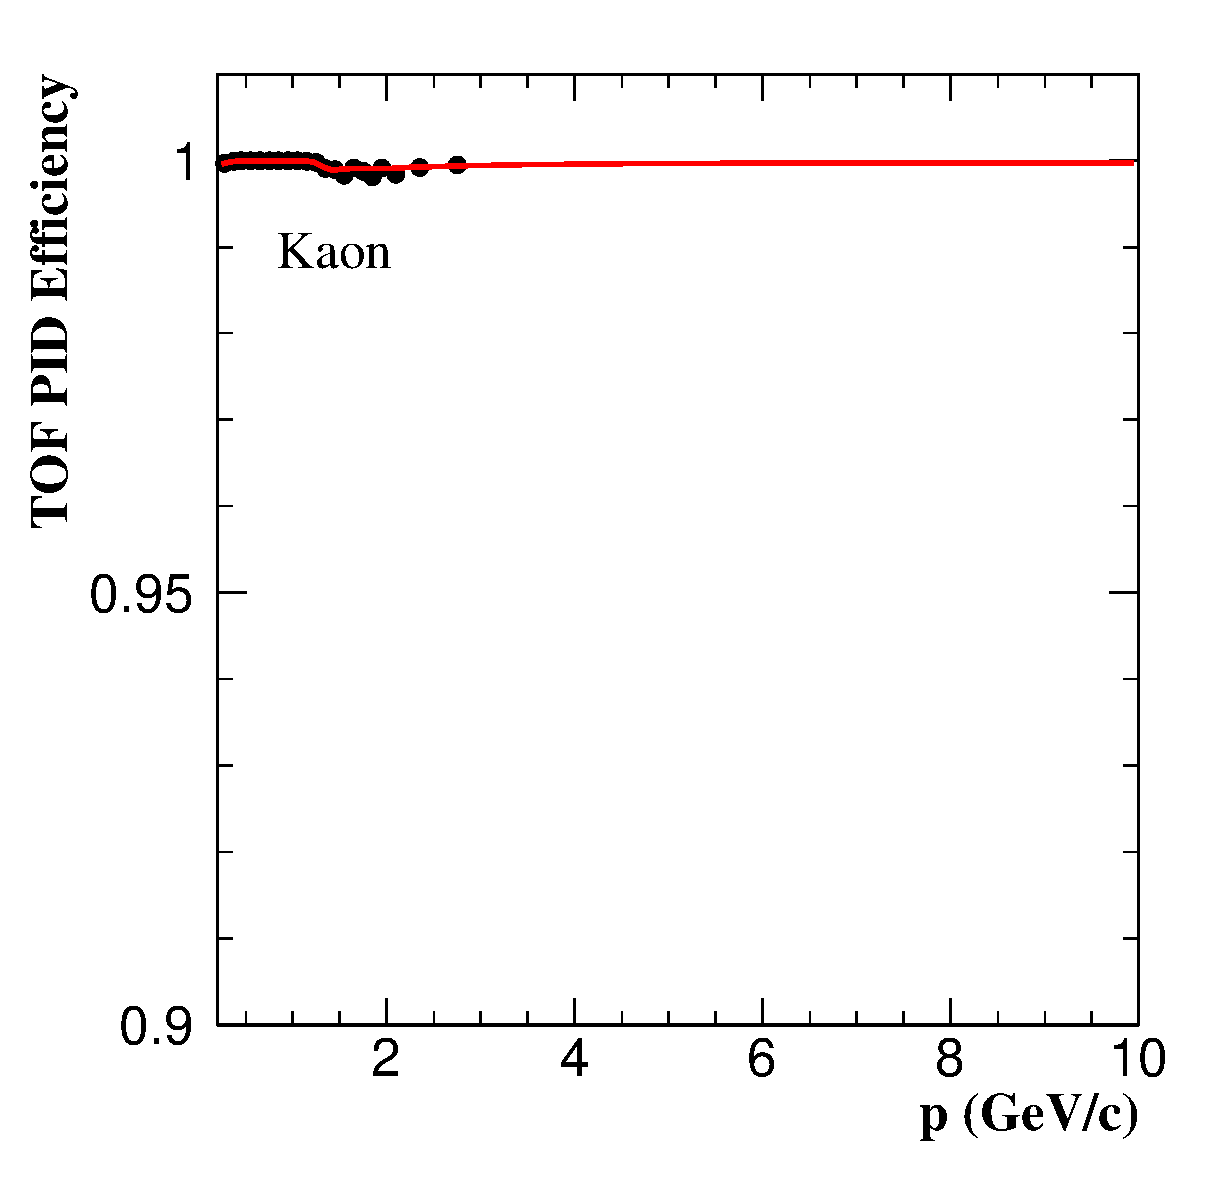
\includegraphics[width=0.47\textwidth]{{figure/Run14TPC/efficiency/kTofPid}.eps}}
    \subfigure{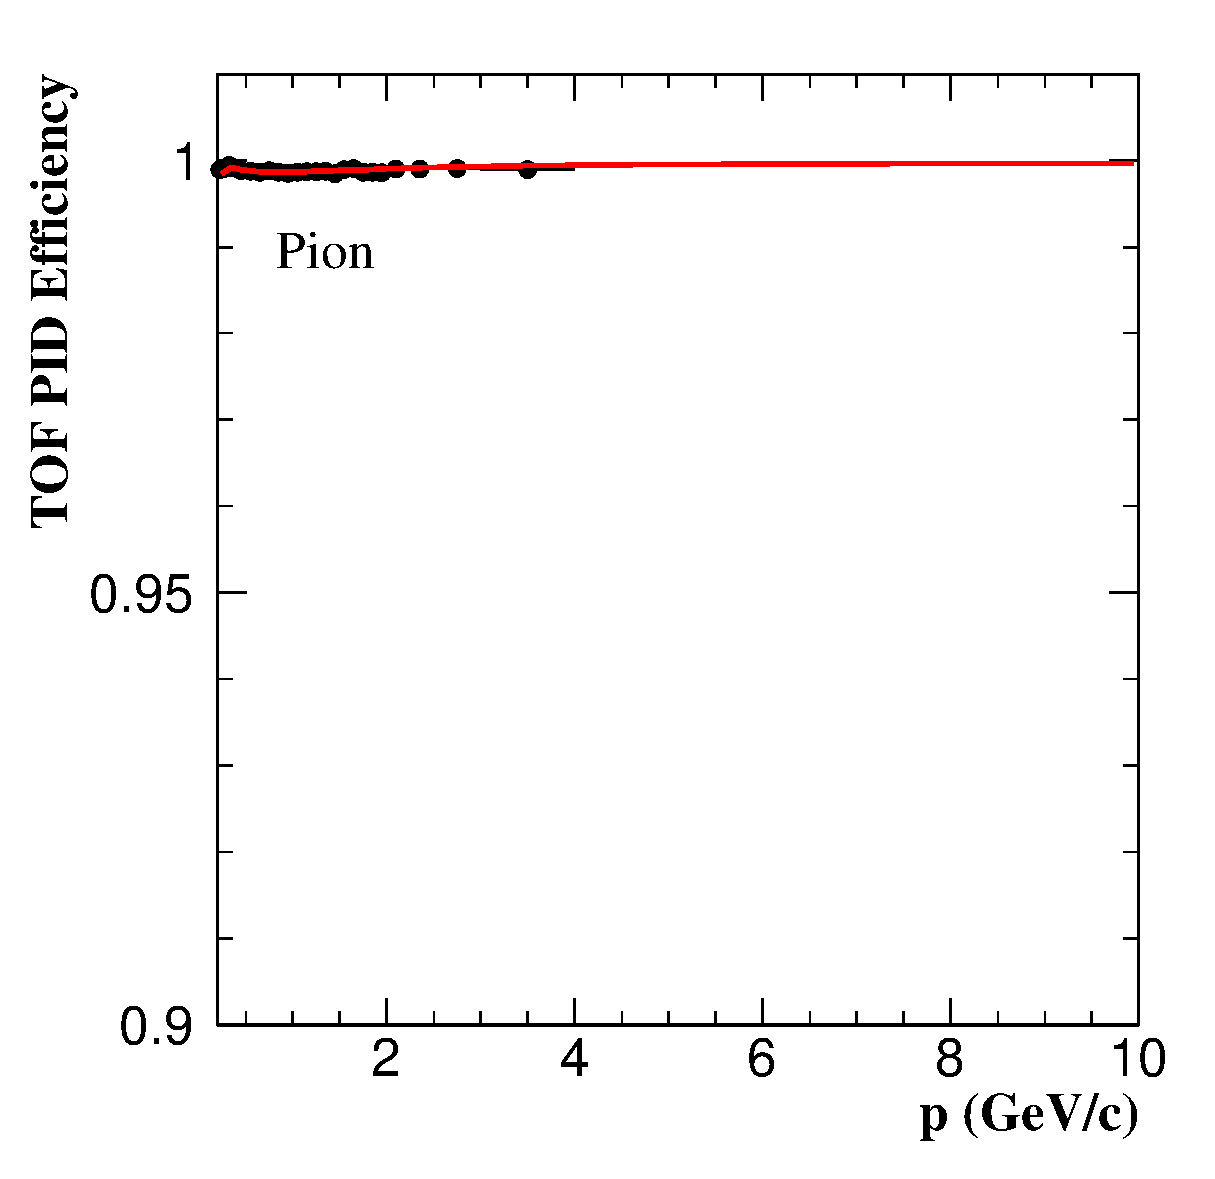
\includegraphics[width=0.47\textwidth]{{figure/Run14TPC/efficiency/piTofPid}.eps}}
    \caption{$K/\pi$ PID efficiency.}
   \label{fig:Run14PidEff}
\end{figure}

Fig.~\ref{fig:Run14singleEff} shows single cut efficiency.
\begin{figure}
    \centering
    \subfigure{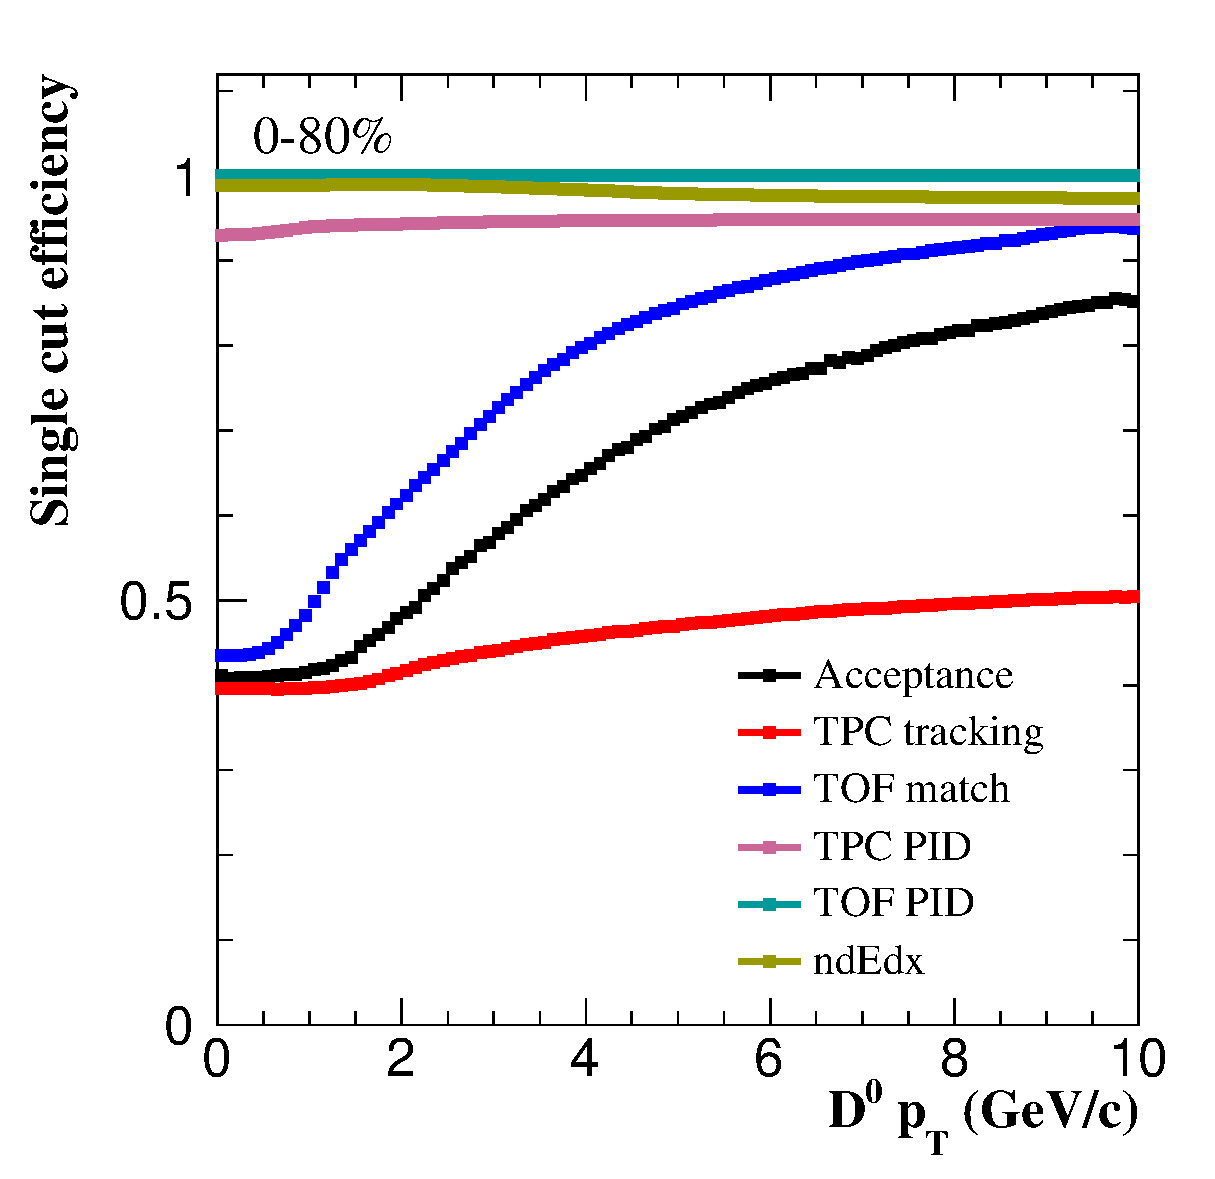
\includegraphics[width=0.5\textwidth]{{figure/Run14TPC/efficiency/SingleCutEff}.eps}}
    \caption{Run14 single cut efficiency.}
   \label{fig:Run14singleEff}
\end{figure}

Fig.~\ref{fig:Run14D0eff} shows final $D^0$ efficiency in two PID cases, left panel for clean PID and right panel for hybrid PID. TPC PID effiency are fixed to be 0.95 both for kaons and pions.
\begin{figure}
    \centering
    \subfigure{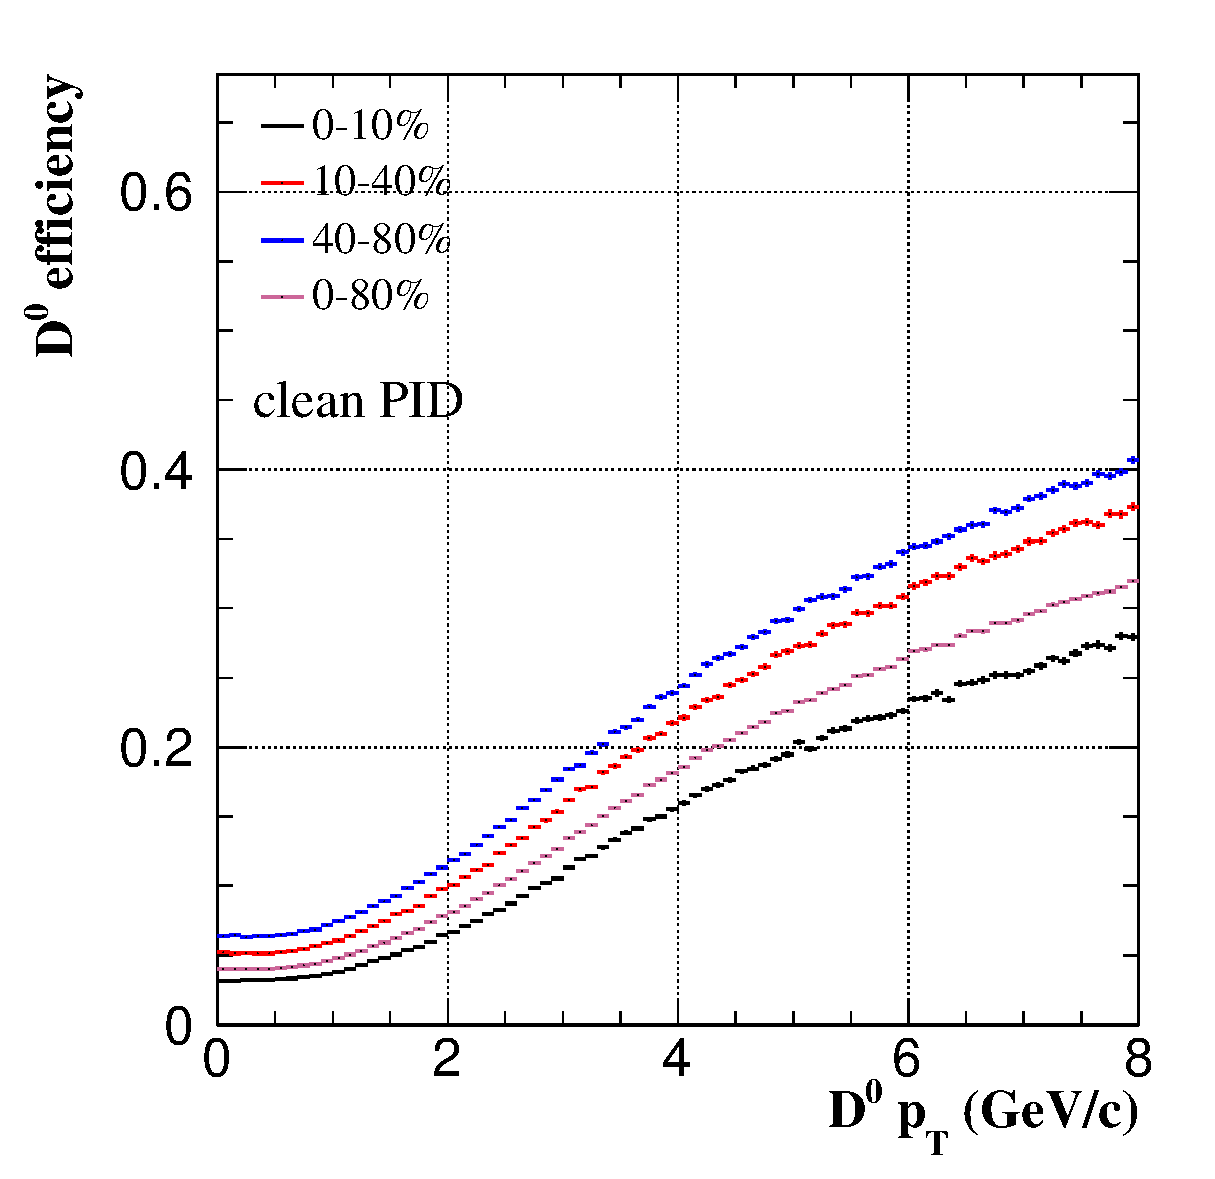
\includegraphics[width=0.47\textwidth]{{figure/Run14TPC/efficiency/Run14_effAll_clean}.eps}}
    \subfigure{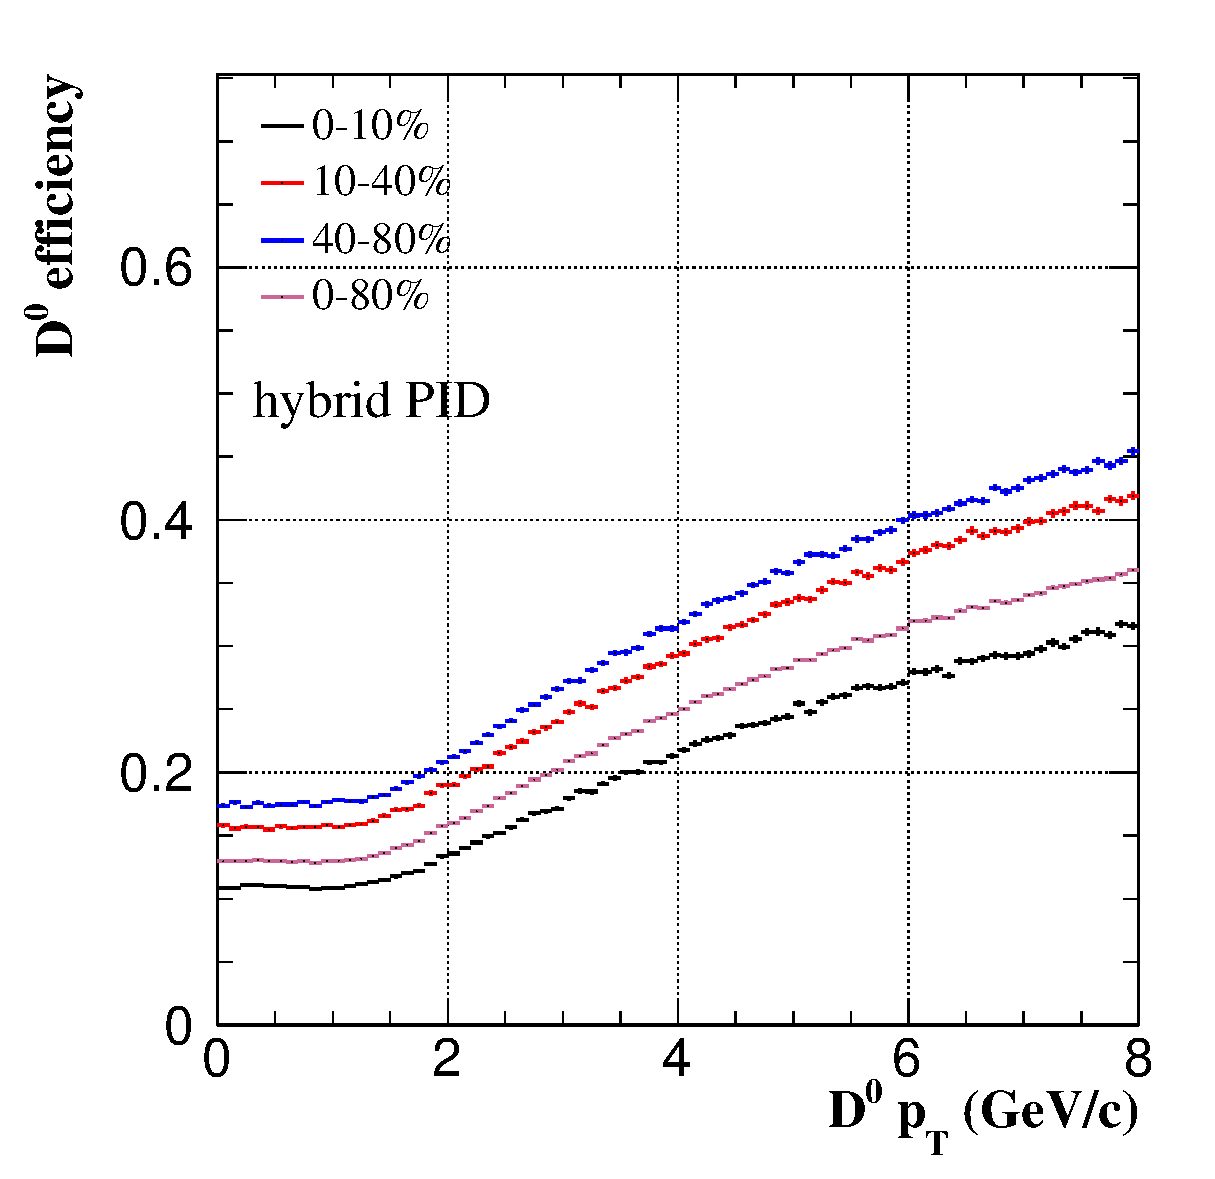
\includegraphics[width=0.47\textwidth]{{figure/Run14TPC/efficiency/Run14_effAll_hybrid}.eps}}
    \caption{Run14 $D^0$ efficiency.}
   \label{fig:Run14D0eff}
\end{figure}

\subsection{Results}
Fig.~\ref{fig:Run14D0} shows $D^0$ spectra comparison between Run14 TPC and Run14 HFT in 6 $p_{T}$ bins. Top panel is $D^0$ spectra and bottom panel is the ratio of Run14 TPC over Run14 HFT. Those data points are removed in which $D^0$ significance is bad ($<$ 3) or $D^0$ width is too narrow ($<$ 9 MeV/$c^2$) or too wide ($>$ 25 MeV/$c^2$). Run14 TPC results are consistent with Run14 HFT results within their statistical errors.
\begin{figure}
    \centering
    \subfigure{\includegraphics[width=0.5\textwidth]{{figure/Run14TPC/ptDivision1/D0Run14_Spectra_0_80}.eps}}
    \caption{$D^0$ spectra comparison between Run14 TPC and Run14 HFT.}
   \label{fig:Run14D0}
\end{figure}

In order to get good $D^0$ significance in different centralities, we also use two wide $p_T$ bins (0-2 and 2-4 GeV/$c$).
Fig.~\ref{fig:Run14D0InCent} shows $D^0$ spectra comparison between Run14 TPC and Run14 HFT in two $p_{T}$ bins. In different centralities, Run14 TPC results are also consistent with Run14 HFT results within their statistical errors.
\begin{figure}
    \centering
    \subfigure{\includegraphics[width=0.45\textwidth]{{figure/Run14TPC/D0Run14_Spectra_0_80}.eps}}
    \subfigure{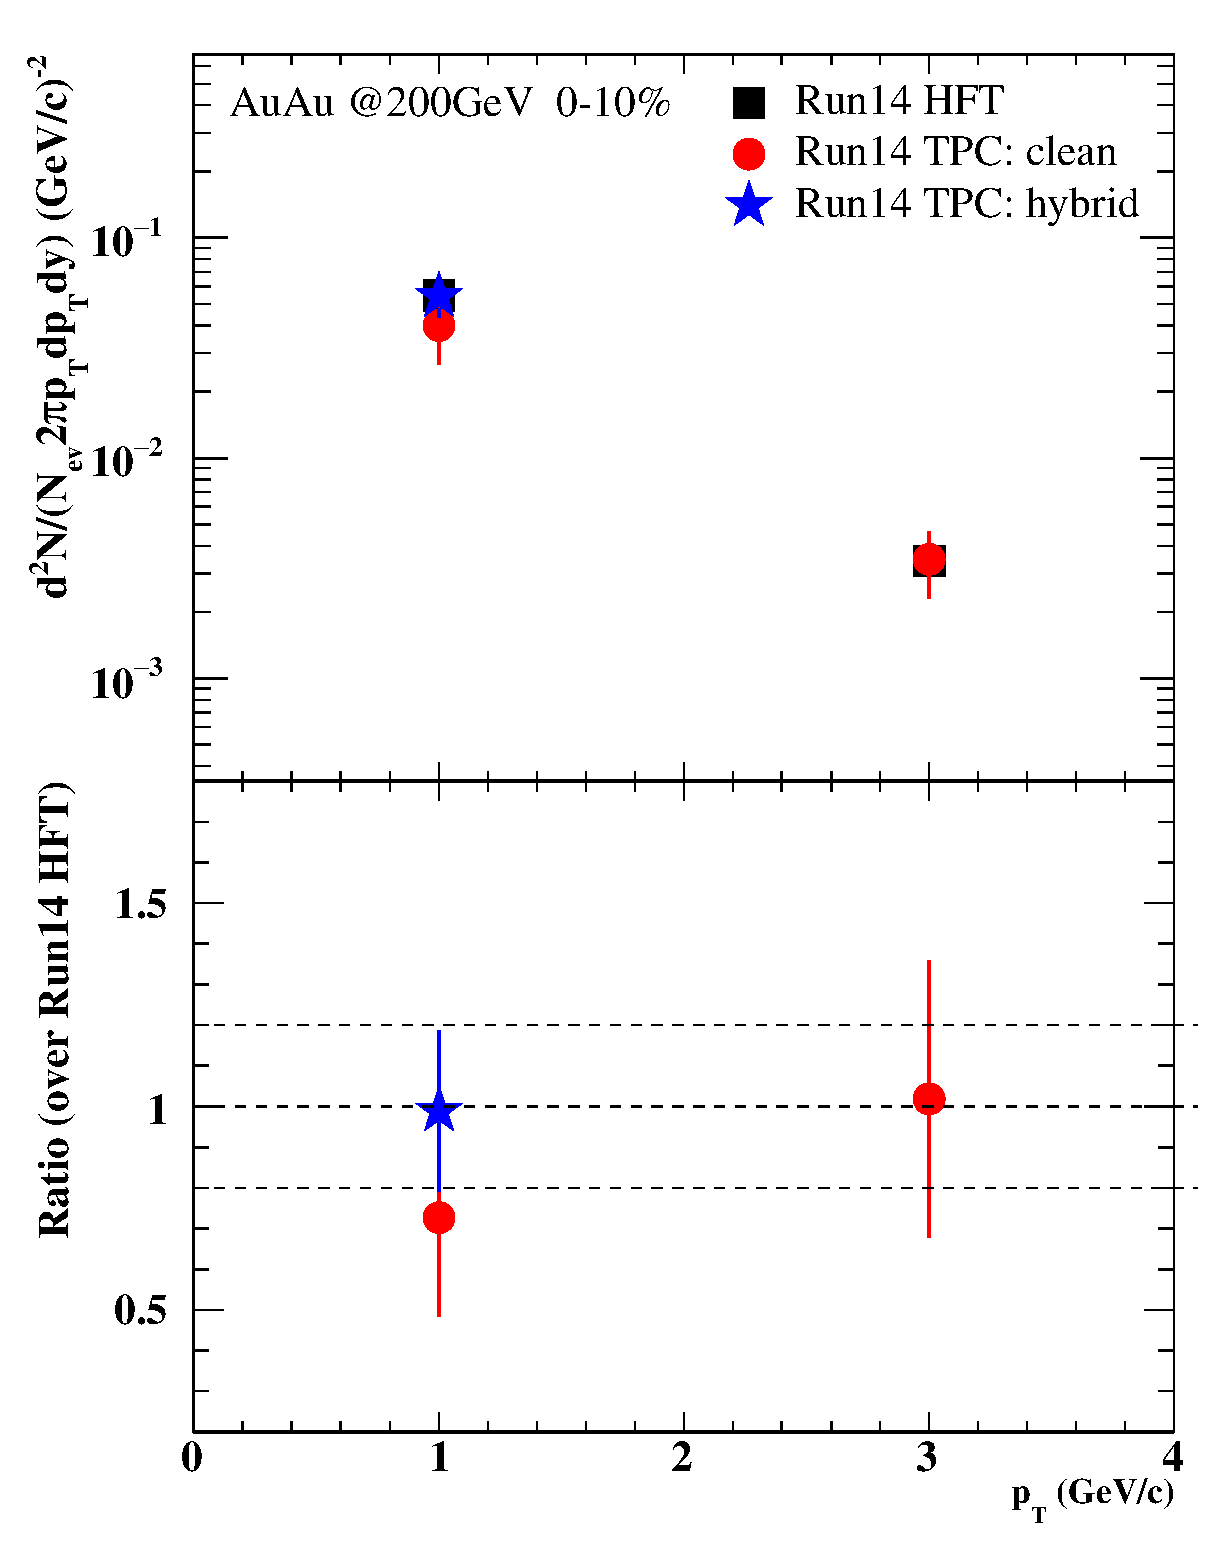
\includegraphics[width=0.45\textwidth]{{figure/Run14TPC/D0Run14_Spectra_0_10}.eps}} \\
    \subfigure{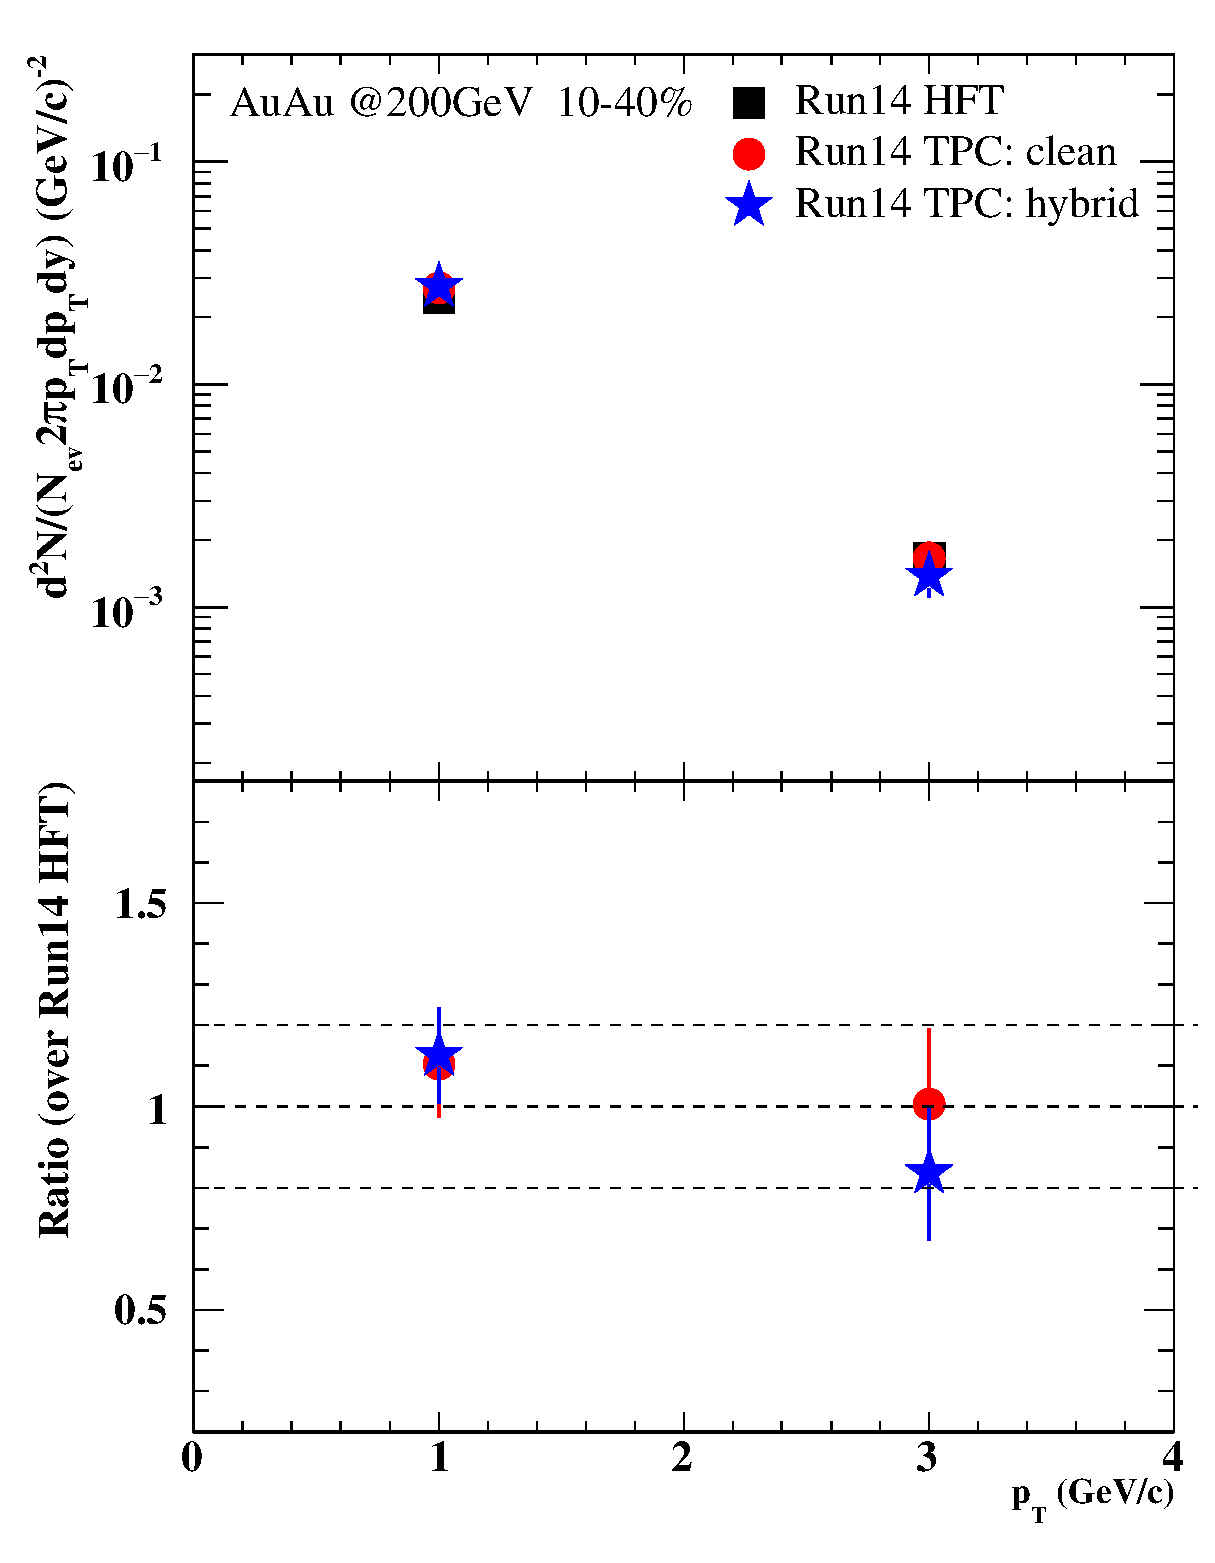
\includegraphics[width=0.45\textwidth]{{figure/Run14TPC/D0Run14_Spectra_10_40}.eps}}
    \subfigure{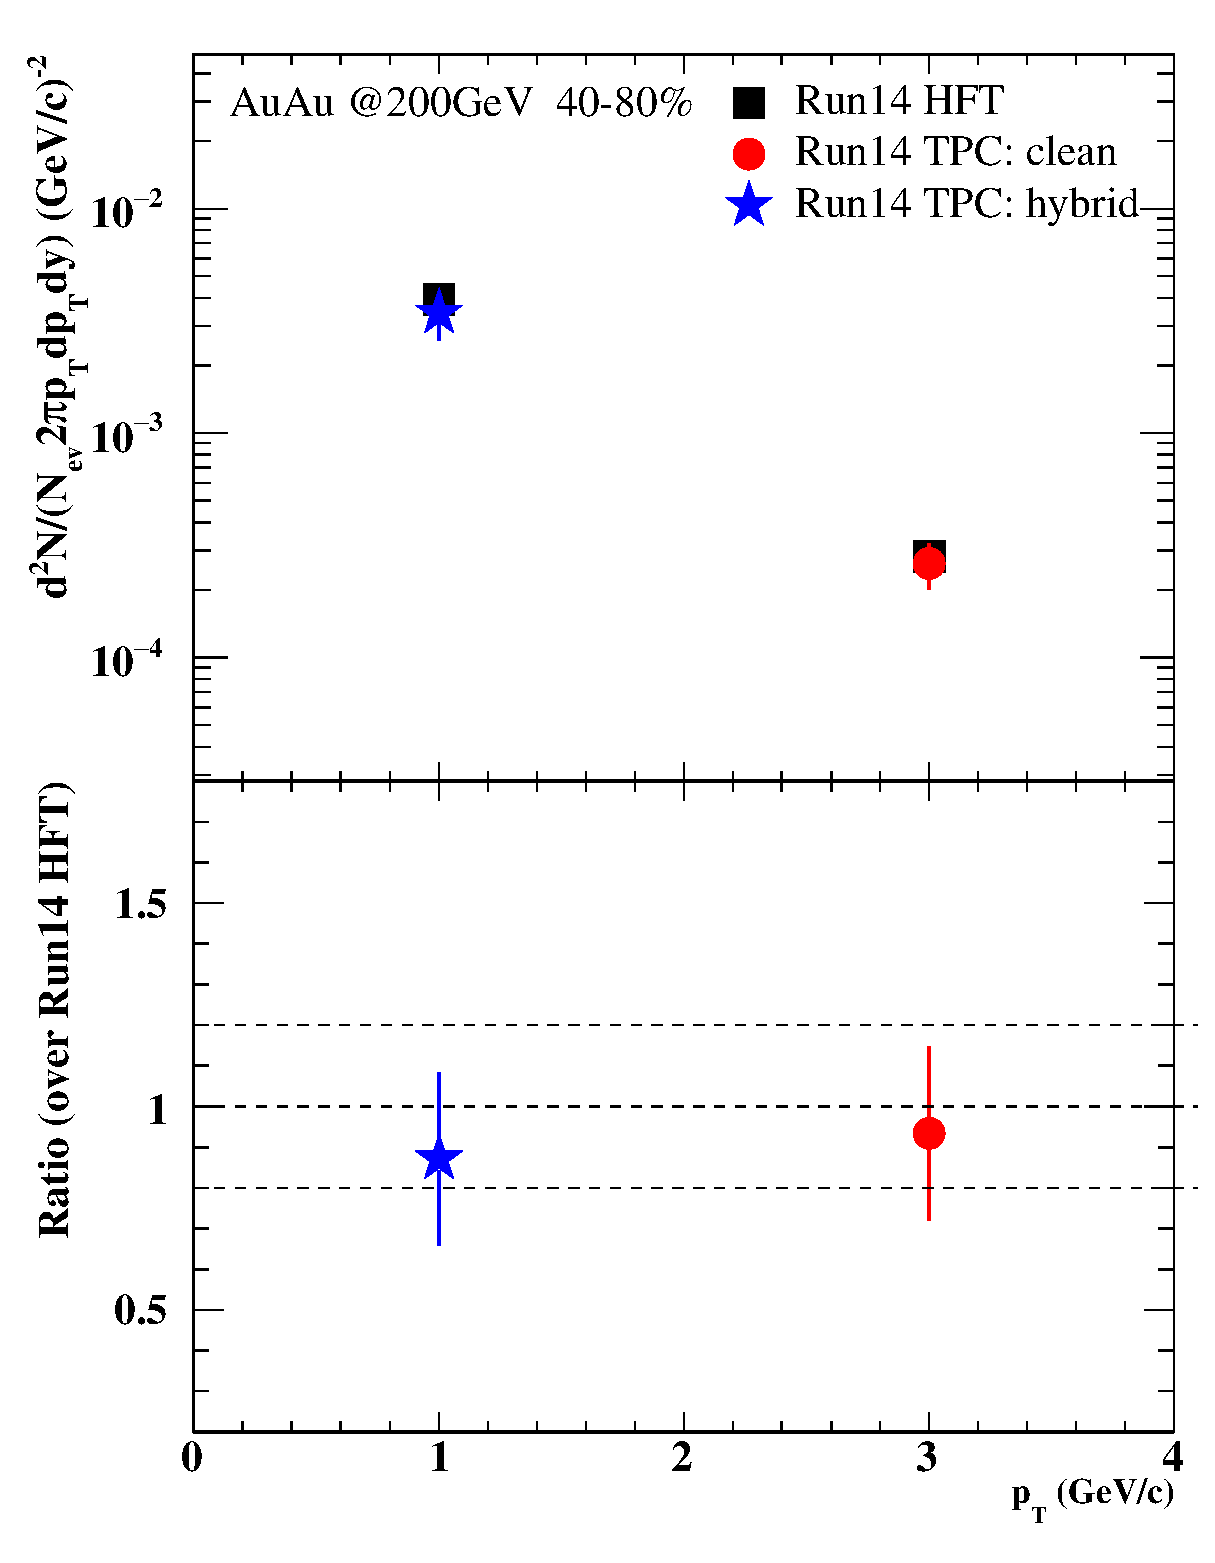
\includegraphics[width=0.45\textwidth]{{figure/Run14TPC/D0Run14_Spectra_40_80}.eps}}
    \caption{$D^0$ spectra comparison between Run14 TPC and Run14 HFT in different centralities.}
   \label{fig:Run14D0InCent}
\end{figure}
